\chapter{Validation croisée des simulations}
Ce chapitre présente seulement les sous-systèmes faisant partie du système intégré et qui permettent de vérifier le cahier des charges.

\section{Convertisseur CC-CC 4 quadrants formé de 2 convertisseurs 3 niveaux NPC}

Le premier sous-système est celui du convertisseur CC-CC 4 quadrants formé de 2 convertisseurs triphasés 3 niveaux NPC avec une commande par MLI à 333Hz, intercalée de 120$^\circ$ par phase. La fréquence vue à la charge est la même que la fréquence de commande de l'AFE, soit 1kHz. L'entrelacement  des commandes permet de réduire les valeurs RMS et moyennes des courants dans les différents bras des convertisseurs. La tension maximale vue des interrupteurs est abaissée à la moitié de la tension du bus CC, ce qui présente un net avantage de dimensionnement. Le sous-système du DCP/DCN permet de remplir l'exigence d'alimenter les électroaimants avec une forme de courant précise. De plus, la puissance moyenne et maximale doivent être similaires à celles prévues par le CERN (18MW crête et 5.4MW moyenne). Les simulations ont été implantées sous SPS et PSIM, le simulateur d'OPAL-RT n'étant pas disponible à temps. Les résultats comparatifs du courant dans la charge sont présentés à la figure \ref{DC_ch_cou_1}. On remarque premièrement que les 2 simulateurs permettent de suivre la consigne de courant demandée. Par la suite, lorsqu'on observe le courant en maintient à 6kA, on remarque qu'il y a une légère différence de fréquence entre les 2 signaux, de l'ordre d'environ 110Hz. La différence est apportée par l'implémentation des filtres dans les 2 simulateurs ainsi que par les algorithmes utilisés afin de solutionner les matrices d'équation d'états (SPS) et les matrices d'admittances nodales (PSIM). De plus, les algorithmes de détection des passages par 0 ne sont pas exactement similaires. SPS utilise une discrétisation par la méthode de Tustin et PSIM une méthode trapézoïdale pure. Ce faisant, vu la quantité de composantes et le nombre de commutations élevées (36 interrupteurs commandés), il est normal d'observer des différences ponctuelles. On constante cependant que les amplitudes observées sont identiques et que les signaux reviennent en phase périodiquement. Les formes d'ondes de courant en montée initiale et en montée rapide permettent de constater que la réponse globale des simulateurs est similaire et qu'ils présentent un comportement analogue.

\paragraph{} La figure \ref{DC_IG_ten_1} présente la tension aux bornes d'un IGBT du DCP/DCN dans les 2 simulateurs. On remarque que les patrons de tensions et les durées de conduction sont identiques. Les amplitudes des tensions aux bornes de l'IGBT le sont aussi. Cependant, qu'il y a un décalage de l'une des simulations par rapport à l'autre, ce qui explique les différences ponctuelles. 

\paragraph{}Pour ce qui est du sous-système formé par le DCP/DCN, on comprend que la commande des interrupteurs représente le fonctionnement désiré, qu'elle permet de remplir l'exigence d'alimenter les électroaimants de l'accélérateur de particules avec une forme de courant précise et une fréquence de modulation équivalente de 1kHz. La puissance instantanée sur 0.9s ainsi que la puissance moyenne mesurée sur 0.9s sont présentées à la figure \ref{DC_IG_ten_2}. On remarque que le critère de puissance maximale (18MW) est respecté ainsi que le critère de puissance moyenne (un peu moins de 5.4MW). Ces critères sont ceux qui ont été fournis par le CERN. Aussi, la correspondance du fonctionnement dans PSIM et dans SPS a été vérifiée par des comparaisons à l'échelle de la modulation. 

\begin{figure}[htb]
\centering
\makebox[\textwidth][c]{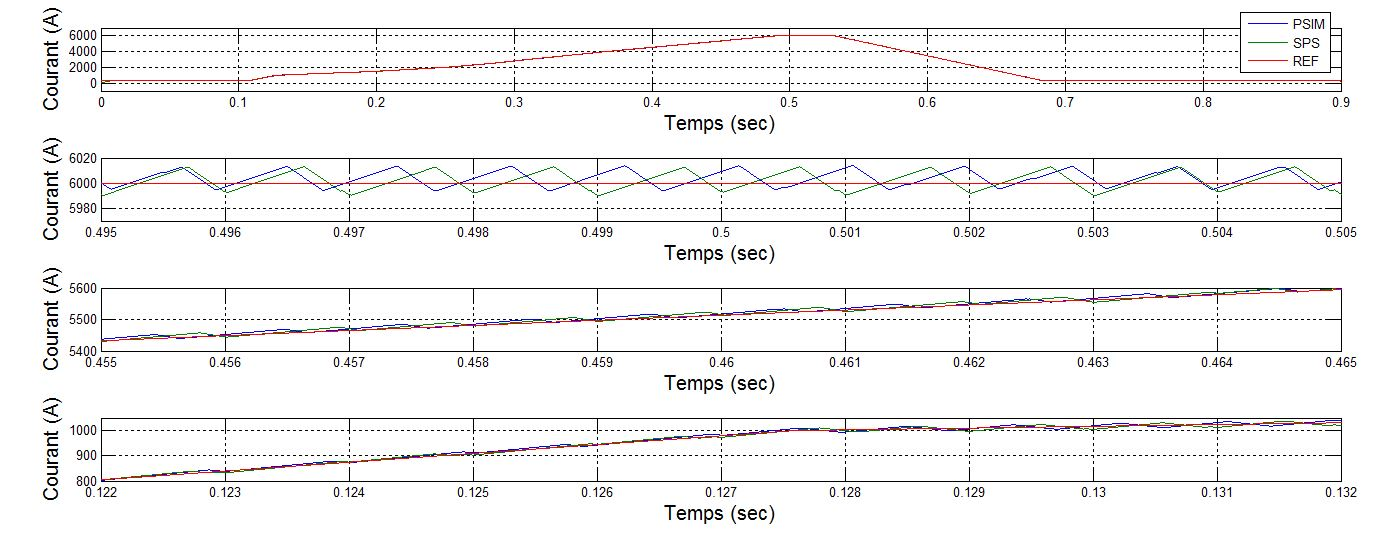
\includegraphics[scale=0.5]{fig/DCPDCN/DCPCourantCharge1u.jpg}}
\caption{Courant traversant la charge sur PSIM et SPS pour un pas de calcul de 1$\mu$s pour le DCP/DCN}
\label{DC_ch_cou_1}
\end{figure}

\begin{figure}[htb]
\centering
\makebox[\textwidth][c]{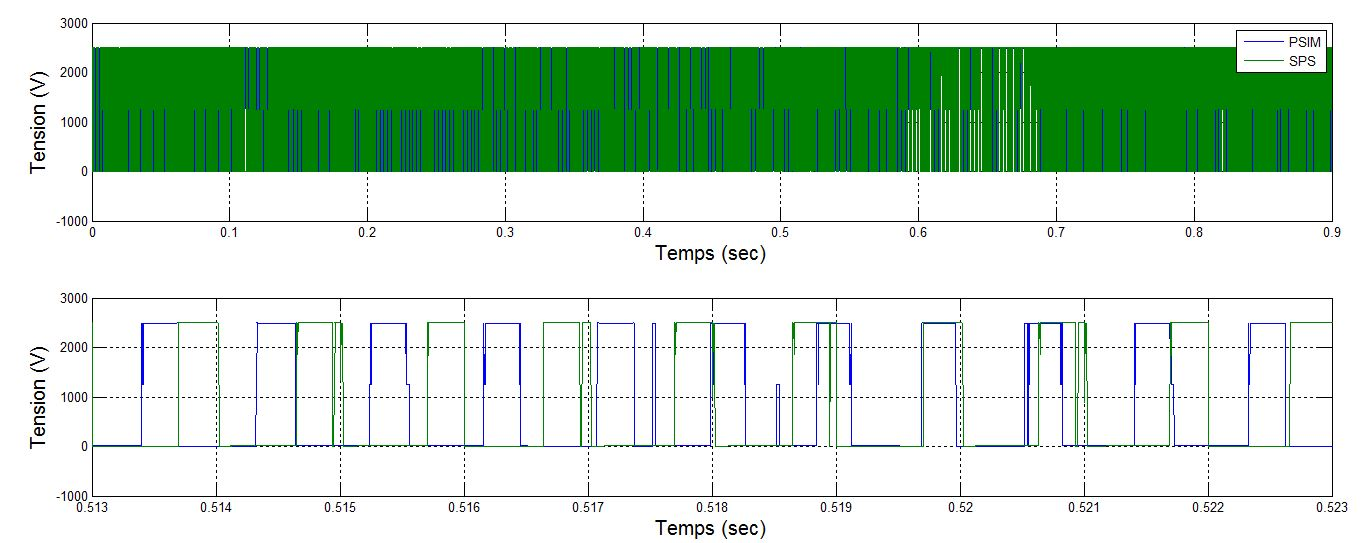
\includegraphics[scale=0.5]{fig/DCPDCN/DCPTensionIGBT1u.jpg}}
\caption{Tension aux bornes d'un IGBT sur PSIM et SPS pour un pas de calcul de 1$\mu$s pour le DCP/DCN}
\label{DC_IG_ten_1}
\end{figure}

\begin{figure}[htb]
\centering
\makebox[\textwidth][c]{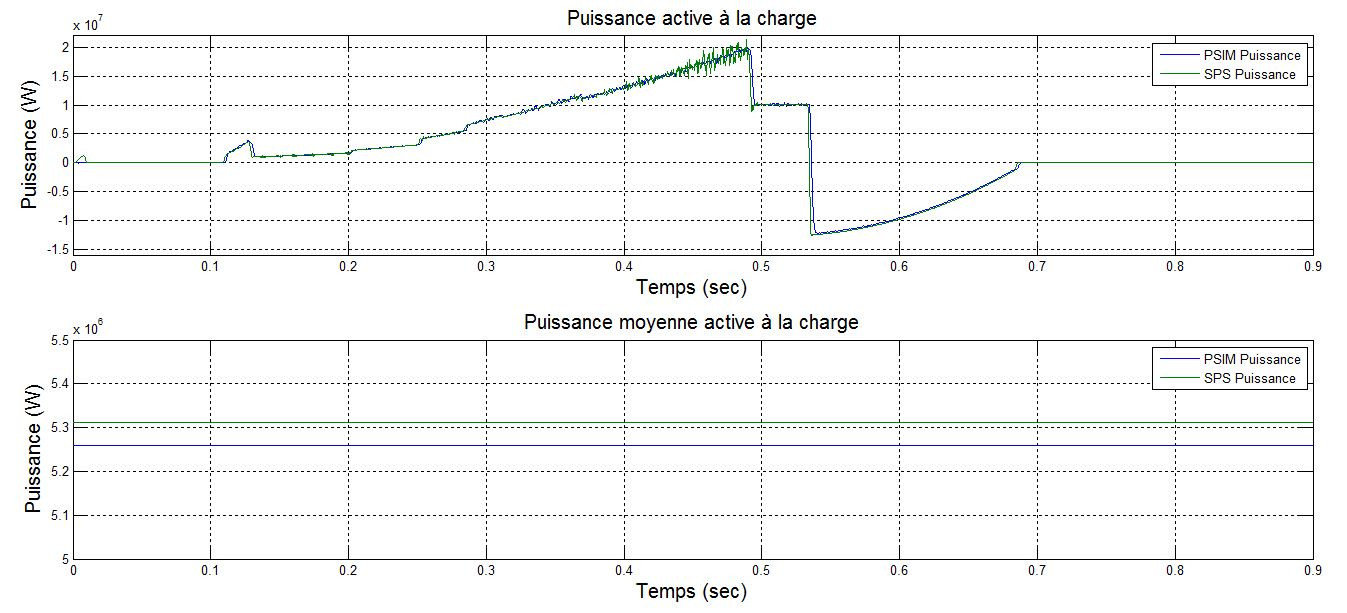
\includegraphics[scale=0.5]{fig/P_DCP.jpg}}
\caption{Puissance active délivrée sur la charge RL sur PSIM et SPS pour un pas de calcul de 1$\mu$s pour le DCP/DCN}
\label{DC_IG_ten_2}
\end{figure}

\clearpage
\section{AFE 3 niveaux NPC avec contrôle par MLI}

Le second sous-système est celui de l'AFE 3 niveaux NPC triphasé avec contrôle par MLI débitant sur une charge RC équivalente. Ce sous-système permet de remplir l'exigence de redresser le signal d'entrée du transformateur, de fournir une puissance moyenne maximale de 2.7MW et une puissance crête maximale de 3.6MW. Cela, tout en maintenant la phase du courant nulle par rapport à la tension. La figure \ref{AF_RC_cou} présente le courant d'entrée pour l'AFE sur charge RC suivant des variations périodiques de la consigne de tension. On cherche ici à présenter la stabilité transitoire et en régime permanent de l'AFE débitant sur une charge RC. L'objectif étant de montrer que les réglages employés donnent des réponses transitoires et permanentes identiques en perturbation. On remarque que les courbes de courant de SPS et de PSIM présentent des réponses pratiquement identiques et indissociables. La figure \ref{AF_RC_ten} présente la tensions aux bornes de la charge RC suivant des variations périodiques de la consigne de tension. On constate que les réponses entre SPS et PSIM sont très similaires et que la tension converge vers la même tension en régime permanent. Par ailleurs, on constate que le courant d'entrée se stabilise suivant une perturbation et que les régulateurs choisis présentent un fonctionnement stable en perturbation. La figure \ref{AF_RC_igbt}
présente la tension et le courant d'un IGBT de l'AFE en régulation suivant des variations périodiques de la consigne de tension. On constate que les simulateurs fournissent des résultats à toutes fins pratiques identiques sur ce point.

\paragraph{}Pour cette section, il est possible de constater que l'AFE remplit le critère de redresser le signal d'entrée avec un courant présentant un déphasage de près de $0^\circ$ avec la tension. Cela peut être confirmé avec la figure \ref{AF_RC_PH} qui présente la phase entre le courant et la tension en régulation de tension. On vérifie la fréquence de commutation en prenant une transformée de fourrier de la tension ligne-ligne vue à l'entrée du redresseur. La figure \ref{AF_RC_ten_L} présente la tension ligne-ligne pour les 2 simulateurs.

\begin{figure}[htb]
\centering
\makebox[\textwidth][c]{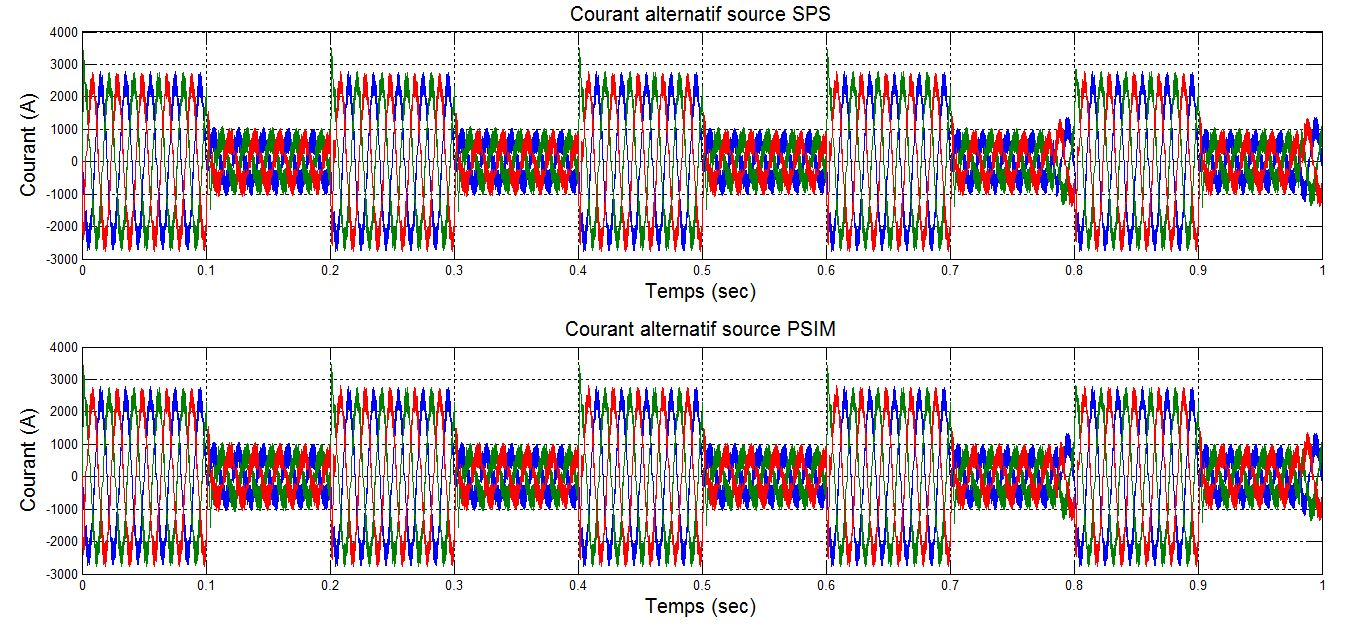
\includegraphics[scale=0.5]{fig/coual_afe.jpg}}
\caption{Courant d'entrée à 1$\mu$s pour l'AFE sur charge RC suivant des variations périodiques de la consigne de tension}
\label{AF_RC_cou}
\end{figure}




\begin{figure}[htb]
\centering
\makebox[\textwidth][c]{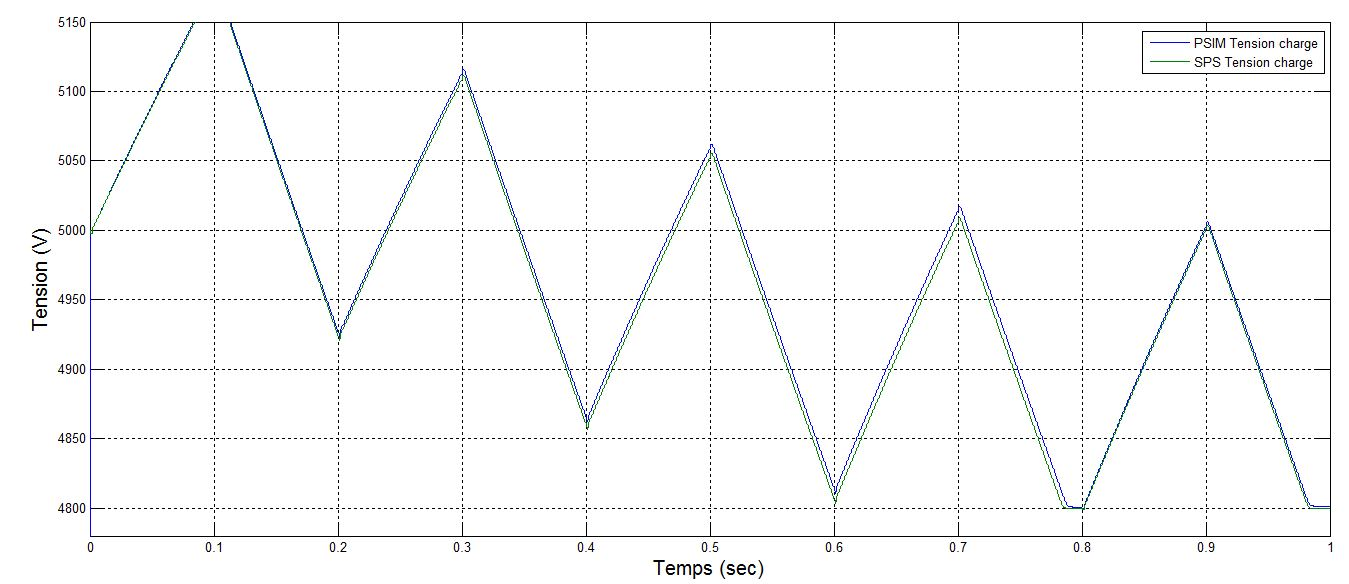
\includegraphics[scale=0.5]{fig/ten_afe.jpg}}
\caption{Tension à la charge à 1$\mu$s pour l'AFE sur charge RC suivant des variations périodiques de la consigne de tension}
\label{AF_RC_ten}
\end{figure}



\begin{figure}[htb]
\centering
\makebox[\textwidth][c]{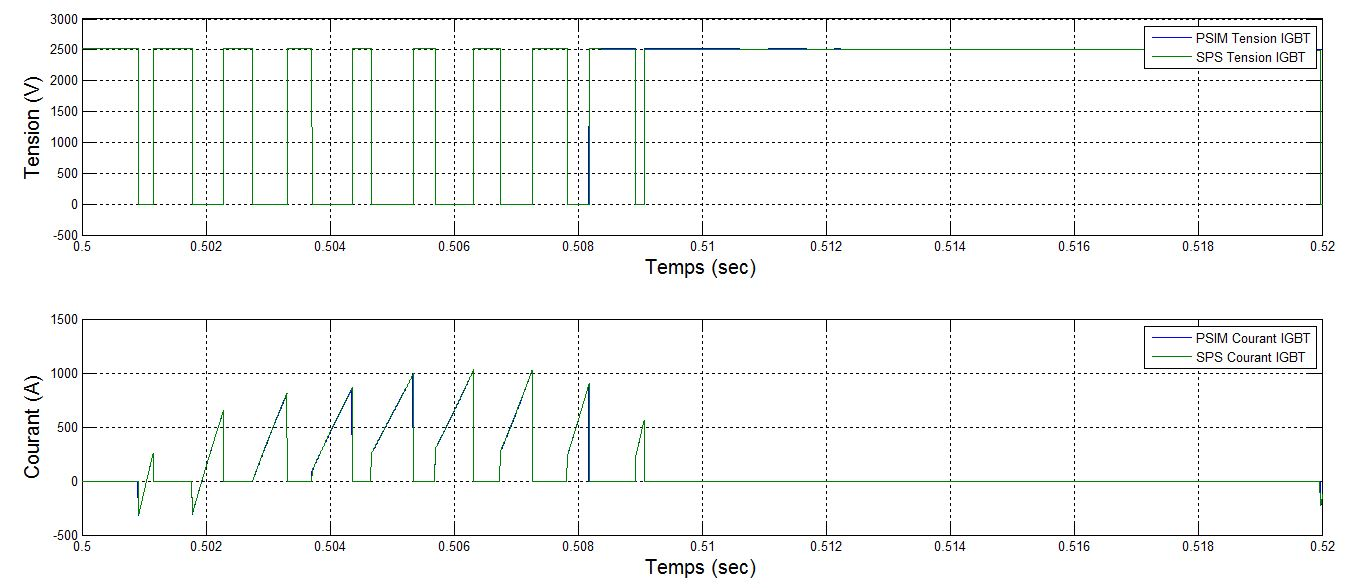
\includegraphics[scale=0.5]{fig/com_afe.jpg}}
\caption{Tension et le courant au bornes d'un IGBT à 1$\mu$s pour l'AFE sur charge RC}
\label{AF_RC_igbt}
\end{figure}

\begin{figure}[htb]
\centering
\makebox[\textwidth][c]{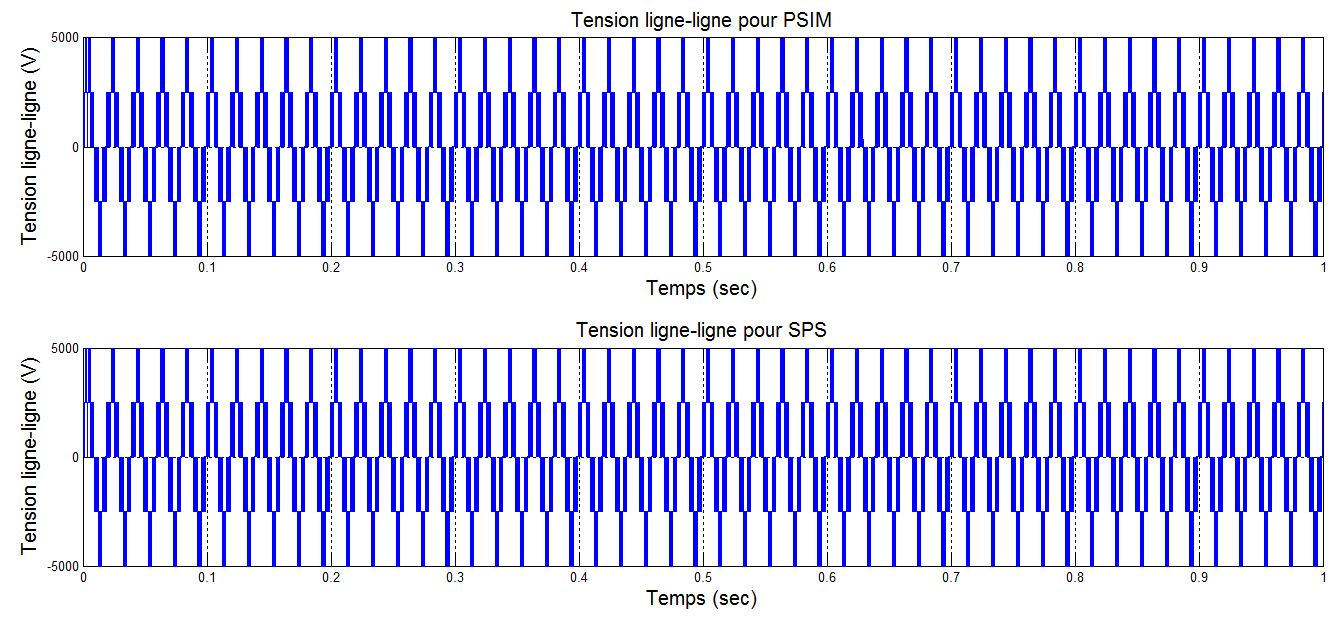
\includegraphics[scale=0.5]{fig/L.jpg}}
\caption{Tension ligne-ligne à 1$\mu$s pour l'AFE sur charge RC sans perturbation}
\label{AF_RC_ten_L}
\end{figure}

\begin{figure}[htb]
\centering
\makebox[\textwidth][c]{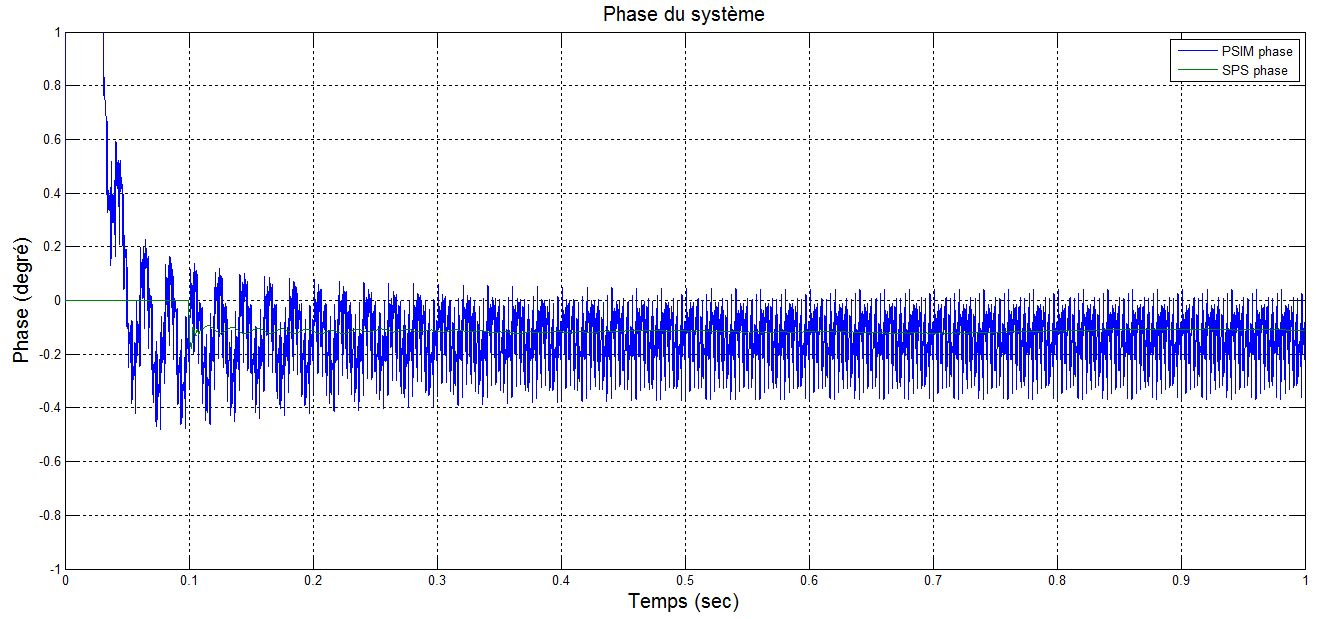
\includegraphics[scale=0.5]{fig/phase.jpg}}
\caption{Phase entre le courant et la tension à 1$\mu$s pour l'AFE sur charge RC sans perturbation}
\label{AF_RC_PH}
\end{figure}


\clearpage
\section{Système intégré: AFE 3 niveaux NPC avec contrôle par MLI avec convertisseur CC-CC formé de 2 cellules NPC 3 niveaux}
Cette section présente le système intégré, soit l'AFE triphasé 3 niveaux NPC avec contrôle par MLI dont la charge est un convertisseur CC-CC formé de 2 cellules onduleur NPC triphasé à 3 niveaux avec une commande par MLI décalée. En ce qui attrait à l'AFE 3 niveaux, la figure \ref{AF_DC_cou1} présente le courant d'entrée du redresseur en fonction du temps. On constate que les formes d'ondes entre SPS et PSIM sont pratiquement identiques et indissociables à l'oeil. La figure \ref{AF_DC_vch1} présente la tension aux bornes de la charge pour un cycle complet sous SPS, PSIM  et selon une courbe de référence extrapolée d'un document fourni par le CERN. La constante de charge du système est identique dans SPS et PSIM et la pente plus abrupte sur la courbe présentée par le CERN. La différence entre les tensions sur SPS et PSIM est au maximum de 50V en descente. On constate que le temps de charge du banc de condensateurs est de 0.28s pour PSIM et de 0.33s pour SPS. Le temps de charge du CERN est autour de 0.28s. L'erreur avec le CERN est autour de 200V, en plus d'une descente plus marquée. Par contre, étant donné que les réglages utilisés ont été réalisés de manière indépendante à ceux effectués au CERN et avec des méthodes totalement différentes, on considère que le système obtenu représente suffisamment bien celui du CERN pour fins de dimensionnement et d'analyse.

\paragraph{}La figure \ref{AF_DC_CHA1} présente le courant à la charge lorsque la tension du bus DC est maintenue par un AFE 3 niveaux. On remarque que l'erreur en maintient est plus constates et que les fréquences ne glissent pas. Cependant, il est possible de constater des perturbations de la forme d'onde sur PSIM, probablement causé par des ré-amorçages d'IGBT. Somme toute, les amplitudes des courants sur les 2 simulateurs sont identiques et l'ondulation  de courant est maintenue inférieure à $\pm$10A. Il est à noter que la précision obtenue au CERN est largement supérieure, mais que nous ne disposons pas de la même souplesse de réglage avec la méthode de régulation implantée. Les courants en montée  et en descente ne présentent pas de différences notables et sont analogues à ceux obtenus sans l'AFE.

\paragraph{} Pour ce qui est de maintenir une puissance maximale autour de 3.6MW et une puissance moyenne de 2.7MW sur un cycle, on constate au moyen de la figure \ref{AF_DC_CHA2} que cet objectif est rempli et que les réglages apportés limitent correctement la puissance à l'entrée. L'ondulation est causée par la présence d'harmoniques dans le signal de courant. Il est à noter un décalage des résultats entre PSIM et SPS. La courbe de SPS étant en retard sur celle de PSIM. Par ailleurs, la puissance moyenne n'est pas exactement à 2.7MW, puisque la méthode de régulation employée dans la conception ne permet pas explicitement d'imposer la puissance de l'AFE en contrôle dynamique. La souplesse possible avec des contrôleurs PID simples ne permet pas d'atteindre cet objectif, il est essentiel d'utiliser une méthode de réglage comparable à celle du CERN pour y arriver.



\begin{figure}[htb]
\centering
\makebox[\textwidth][c]{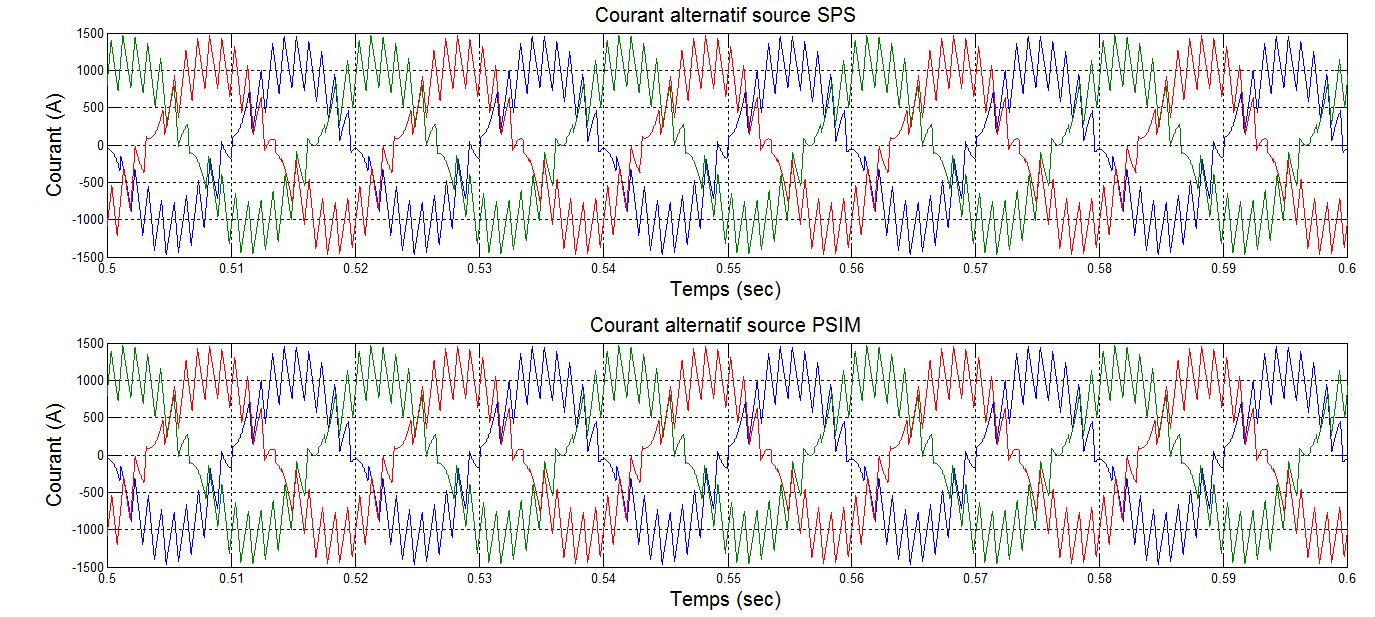
\includegraphics[scale=0.5]{fig/DCP_AFE/1u/cour_al.jpg}}
\caption{Courant d'entrée de l'AFE pour un pas de calcul de 1$\mu$s}
\label{AF_DC_cou1}
\end{figure}


\begin{figure}[htb]
\centering
\makebox[\textwidth][c]{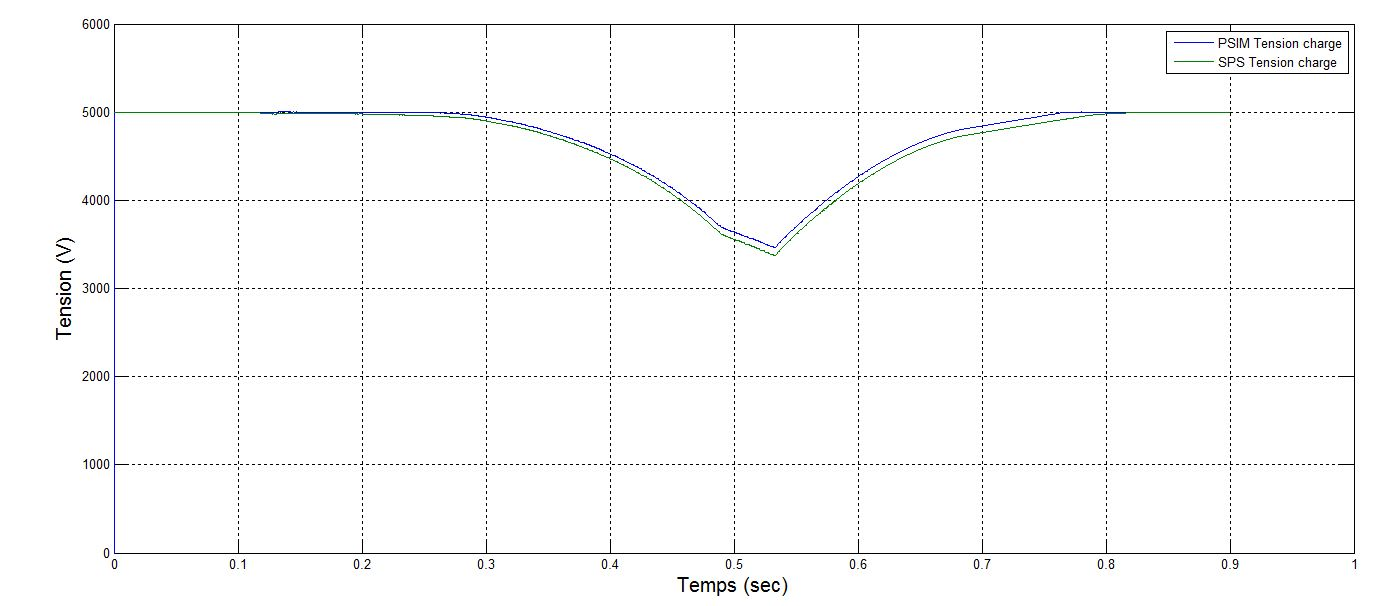
\includegraphics[scale=0.5]{fig/DCP_AFE/1u/ten_bus.jpg}}
\caption{Tension du bus CC pour un pas de calcul de 1$\mu$s}
\label{AF_DC_vch1}
\end{figure}

\begin{figure}[htb]
\centering
\makebox[\textwidth][c]{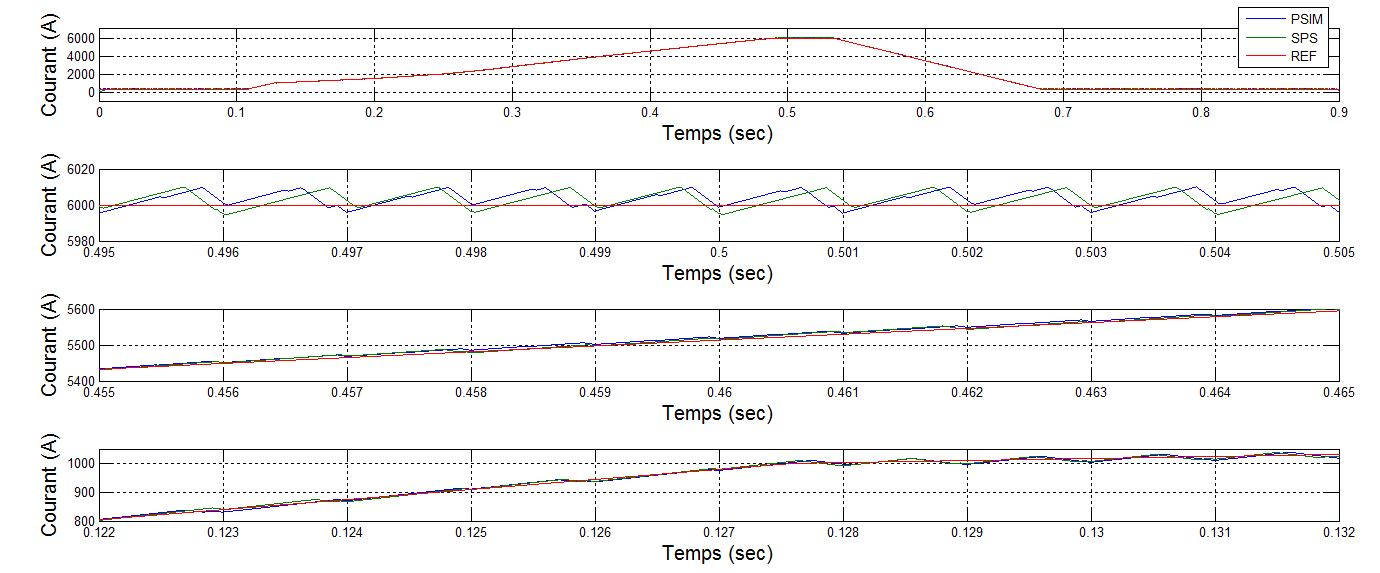
\includegraphics[scale=0.5]{fig/DCP_AFE/1u/cour_ch.jpg}}
\caption{Courant aux bornes des électroaimants pour un pas de calcul de 1$\mu$s}
\label{AF_DC_CHA1}
\end{figure}

\begin{figure}[htb]
\centering
\makebox[\textwidth][c]{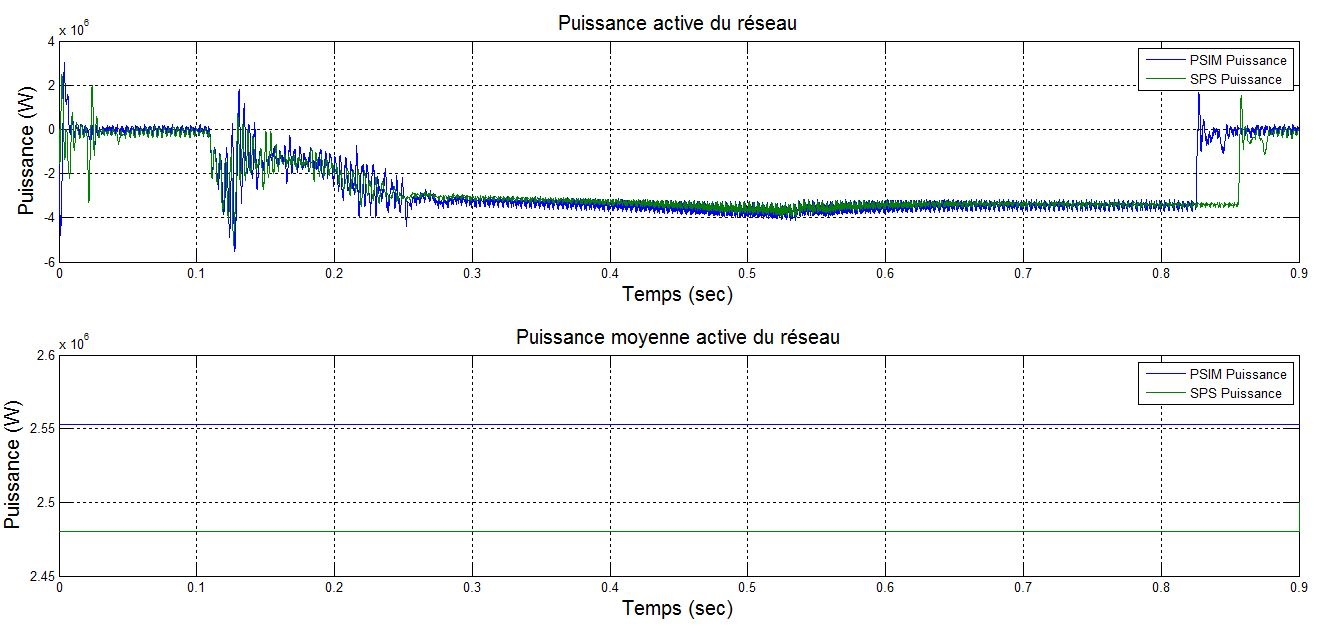
\includegraphics[scale=0.5]{fig/DCP_AFE/1u/PUI.jpg}}
\caption{Puissance délivrée par le réseau alternatif pour un pas de calcul de 1$\mu$s}
\label{AF_DC_CHA2}
\end{figure}


\section{Comparatif des temps de simulation}
Les temps de simulation de l'ensemble des sous-systèmes qui ont été implanté dans les simulateurs sur les 2 plateformes sont résumés au tableau \ref{tab_temps_simulation}. Ce tableau présente les temps totaux de simulation pour 2 ordinateurs munis de processeurs différents. L'objectif est de vérifier la complexité algorithmique relative des 2 plateformes de simulation. On note que les simulations de complexité croissante provoquent un impact plus marqué sur le temps de calcul sur PSIM que sur SPS. 
\begin{table}[h]
\centering
\begin{tabular}{|l||c|c|c|c|c|}
\hline
&  \multicolumn{2}{>{\centering\arraybackslash}m{1.2in}|}{Intel Core 2 Duo T9900 3.06GHz}        & \multicolumn{2}{c|}{AMD FX-8350 4 GHz}               \\\hline
Simulations                      & SPS                       & PSIM  & SPS    & PSIM   \\
AFE 3 LEVEL+DCP/DCN 0.9sec       & 22min                     & 23min & 5m 54s & 7m 23s \\
AFE 2 LEVEL + HACHEUR 0.9sec     & 5min                      & 5min  & 3m 08s & 1m 28s \\
AFE 3 LEVEL PWM 1sec             & 9min                      & 5min  & 4m 11s & 1m 41s \\
AFE 2 LEVEL HYSTERESIS 1sec      & 7min                      & 4min  & 2m 33s & 1m 19s \\
AFE 2 LEVEL IDEAL 1sec           & 8min                      & 6min  & 2m 49s & 2m 5s  \\
DCP/DCN 0.9sec                  & 5min                      & 5min  & 2m 48s & 1m 41s \\
HACHEUR 4 QUADRANTS 0.9sec       & 3min                      & 1min  & 1m 20s & 16s \\ \hline 
\end{tabular}
\caption{Résumé des temps de simulations sur 2 ordinateurs munis de processeurs différents}
\label{tab_temps_simulation}
\end{table}



